\documentclass[border=5mm,tikz]{standalone}
\usepackage{tikz}
\usetikzlibrary{positioning}
\begin{document}

  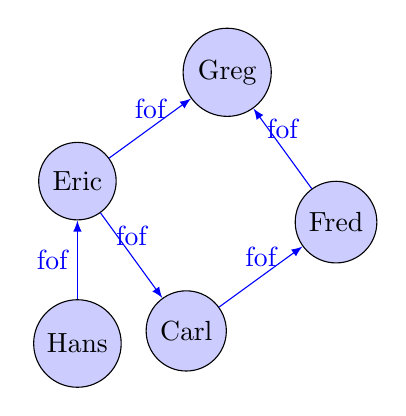
\begin{tikzpicture}
    \foreach \ang/\lab/\User in {0/C/Carl,72/E/Eric} {
      \node[circle,fill=blue!20,draw] (\lab) at (\ang:2){\User};
    }
    %\path[-latex,blue] (A) edge [above] node [blue] {fof} (B);
    %\path[-latex,blue] (A) edge [above] node [blue] {fof} (C);
    %\path[-latex,blue] (B) edge [above] node [blue] {fof} (D);
    %\path[-latex,blue] (E) edge [above] node [blue] {fof} (D);
    \path[-latex,blue] (E) edge [above] node [blue] {fof} (C);
    \node[circle,fill=blue!20,draw] (F) at (19.5:4.14){Fred};
    \node[circle,fill=blue!20,draw] (G) at (52.5:4.14){Greg};
    \node[circle,fill=blue!20,draw,below=of E] (H) {Hans};
    \path[-latex,blue] (C) edge [above] node [blue] {fof} (F);
    \path[-latex,blue] (F) edge [above] node [blue] {fof} (G);
    \path[-latex,blue] (E) edge [above] node [blue] {fof} (G);
    \path[-latex,blue] (H) edge [left] node [blue] {fof} (E);
  \end{tikzpicture}

\end{document}
